\documentclass{article}%
\usepackage[T1]{fontenc}%
\usepackage[utf8]{inputenc}%
\usepackage{lmodern}%
\usepackage{textcomp}%
\usepackage{lastpage}%
\usepackage[head=40pt,margin=0.5in,bottom=0.6in]{geometry}%
\usepackage{graphicx}%
%
\title{\textbf{Trasladan a Simonovis nuevamente a su casa tras una revisión médica en el Sebin}}%
\author{JOSÉ SILVA}%
\date{21/11/2018}%
%
\begin{document}%
\normalsize%
\maketitle%
\textbf{URL: }%
http://www.eluniversal.com/politica/26313/trasladan{-}a{-}simonovis{-}sin{-}orden{-}judicial{-}a{-}la{-}sede{-}del{-}sebin{-}en{-}plaza{-}venezuela\newline%
%
\textbf{Periodico: }%
EU, %
ID: %
26313, %
Seccion: %
politica\newline%
%
\textbf{Palabras Claves: }%
NO\_TIENE\newline%
%
\textbf{Derecho: }%
1.2%
, Otros Derechos: %
NO\_TIENE%
, Sub Derechos: %
1.2.2%
\newline%
%
\textbf{EP: }%
NO\newline%
\newline%
%
\textbf{\textit{María del Pilar Pertíñez, esposa y defensa del excomisario del Cicpc, indicó que efectivos del Sebin "fuertemente armados" se lo llevaron al alegar que le harían una evaluación en la Torre Venezuela}}%
\newline%
\newline%
%
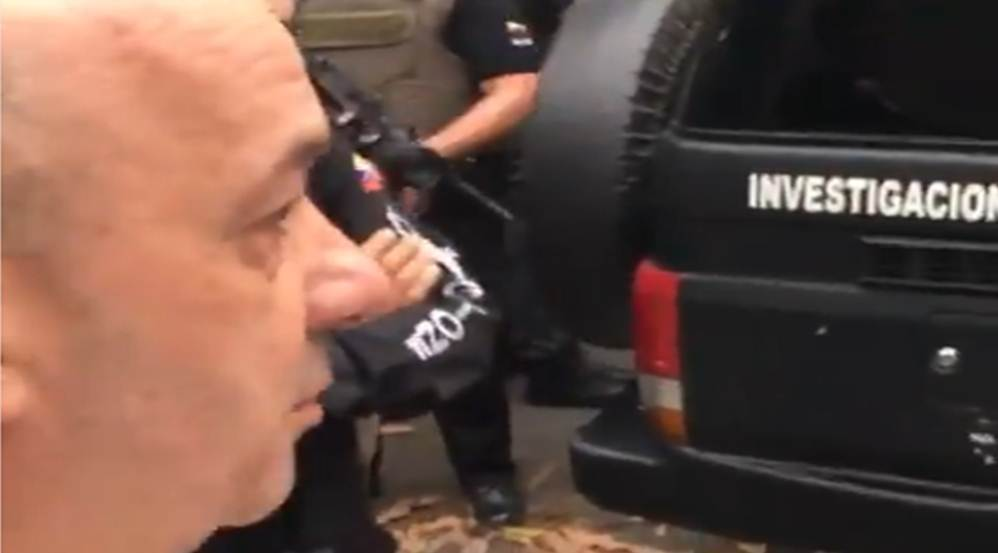
\includegraphics[width=300px]{128.jpg}%
\newline%
%
Caracas.{-} El excomisario del Cicpc, Iván Simonovis, –que cumple arresto domiciliario– fue devuelto a su casa luego de haber sido trasladado la mañana de este miércoles "sin orden judicial" a la sede del Sebin ubicada en Plaza Venezuela, informó su esposa y abogada defensora, María del Pilar Pertíñez, conocida comúnmente como "Bony".%
\newline%
%
”Mi familia no confía en los médicos del Sebin. Iván tiene sus médicos particulares que siempre lo han atendido y son los únicos que pueden determinar el diagnóstico de Iván”, señaló este miércoles Pertíñez en declaración a los medios.%
\newline%
%
La también activista en DDHH aseguró que la nueva directiva del Sebin se encuentra trasladando a los denominados presos políticos hacia la sede del organismo de inteligencia para realizarles evaluaciones médicas.%
\newline%
%
Más temprano, Pertíñez publicó un video en Twitter donde denunció que~"vinieron cuatro carros policiales con funcionarios fuertemente armados, se lo llevaron (a Simonovis), dijeron que iban a hacerle una evaluación en la Torre Venezuela.  Les pedí que me extendieran la orden del tribunal, no lo hicieron".%
\newline%
%
\end{document}